
\documentclass[landscape]{slides}

% Are all these packages really necessary?
\usepackage{times}
\usepackage{ifthen}
\usepackage{amsmath}
\usepackage{amssymb}
\usepackage{amstext}
\usepackage[latin1]{inputenc}
\usepackage{moreverb}
\usepackage{stmaryrd}
\usepackage{url}
\usepackage{epsfig}
\usepackage{mathrsfs}
\usepackage[english]{fp-autoref}
\usepackage{fp-frame}
\usepackage{mathpartir}
\usepackage{enumerate}
\usepackage{listings}
\usepackage{graphics}

\input{slide-macros}
%%%%%%%%%%%%%%%%%%%%%%%%%%%%%%%%%%%%%%%%%%%%%%%%%%%%%%%%%%%%%%%%%%%%%%%%%%%%
% FILE    : macros.tex
% AUTHOR  : (C) Copyright 2013 by Peter C. Chapin
% SUBJECT : Various macro definitions that can be used in my dissertation.
%%%%%%%%%%%%%%%%%%%%%%%%%%%%%%%%%%%%%%%%%%%%%%%%%%%%%%%%%%%%%%%%%%%%%%%%%%%%

\newtheorem{condition}{Condition}[section]
\newtheorem{conject}{Conjecture}[section]
\newtheorem{corollary}{Corollary}[section]
\newtheorem{definition}{Definition}[section]
\newtheorem{example}{Example}[section]
%\newtheorem{exmp}{Example}[section]
\newtheorem{lemma}{Lemma}[section]
\newtheorem{proposition}{Proposition}[section]
\newtheorem{theorem}{Theorem}[section]

\def\arr#1{\textup{\textbf{[}}\mskip -.5mu\textup{\textbf{|}}\, #1 \,\textup{\textbf{|}}\mskip -.5 mu\textup{\textbf{]}}}
\def\blockno{m}
\def\blok#1{\textbf{(}#1\textbf{)}}
\def\castto#1#2{(#1)\,#2}
\def\defassign{::=}
\def\dom{{\rm Dom}}
\def\envletter{E}
\def\figsize{\small}                      % Use in figures to set the size of the figure.
\def\fundef#1{\mathit{#1}}
\def\lc{\textup{\textbf{\{}}}             % Set brackets used in code.
\def\mapidx#1{{(\mskip -2.5mu #1\mskip -2.5mu)}}
\def\maploosemerge{\curlyveedownarrow}
\def\margs#1{\mathrm{<}#1\mathrm{>}}
\def\neight{n^{8}}
\def\nsixtn{n^{16}}
\def\ran{{\rm Ran}}
\def\rc{\textup{\textbf{\}}}}
\def\s{\varsigma}
\def\t{\tau }
\def\undefv{\ttbf{uninit}}
\def\VAR{\textit{x} }

\newcommand{\abs}[1]{|#1|}
\newcommand{\activation}[2]{#1\,\mathit{as}\,#2}
\newcommand{\addt}{\mathit{add}}
\newcommand{\bit}{\ttbf{bit}}
\newcommand{\blockmem}{M}
\newcommand{\bm}{\blockmem}
\newcommand{\bn}{\blockno}
\newcommand{\bootload}{\fundef{bootload}}
\newcommand{\bootseq}[1]{\mathbf{boot}(#1)}
\newcommand{\cast}[2]{\tt{(#1)#2}}
\newcommand{\cedge}[1]{\stackrel{#1}{\longleftarrow}}

% The \code macro should only be used when italic font is needed in inline code snippets, for
% example to deal with metavariables in code examples. Otherwise the listings package should
% be used (the short inline form should be turned on in most chapters). The listings package
% is more configurable and automatically bolds keywords.
\newcommand{\code}[1]{\texttt{#1}}

\newcommand{\codt}[1]{\llbracket #1 \rrbracket}
\newcommand{\compatible}[2]{\mathit{compatible}(#1,#2)}
\newcommand{\compute}{\leadsto}
\newcommand{\context}[2]{#1\lc#2\rc}
\newcommand{\cred}[3]{\mathit{#1} \cedge{#3} \mathit{#2}}
\newcommand{\creds}{\mathcal{C}}
\newcommand{\CT}{{CT}}
\newcommand{\cval}[2]{\lfloor #1,#2 \rfloor}
\newcommand{\datalogc}{$\text{Datalog}_\mathcal{C}$}
\newcommand{\datalog}{\text{Datalog}}
\newcommand{\decl}{d}
\newcommand{\decls}{\vect{\decl};}
\newcommand{\defeq}{\triangleq}
\newcommand{\defvec}[2]{\vect{#1} = \vect{#2}}
\newcommand{\delcred}[3]{#1 \stackrel{#3}{\longrightarrow} #2}
\newcommand{\docast}[3]{\fundef{docast}(#1,#2,#3)}
\newcommand{\exportsty}{\varepsilon}
\newcommand{\exports}{\xi}
\newcommand{\fdname}{\textsf{l}}
\newcommand{\fields}[1]{\mathit{fields}(\tt{#1})}
\newcommand{\fieldvec}[2]{\ttvec{#1}\ \ttvec{#2}}
\newcommand{\filename}[1]{\texttt{#1}}    % File names.
\newcommand{\flash}{F}
\newcommand{\fml}{\ensuremath{\langle \text{ML} \rangle}}
\newcommand{\fname}{\textsf{f}}
\newcommand{\fsub}{\ensuremath{F_\le}}
\newcommand{\gbounds}[2]{\ttvec{#1} <: {\ttvec{#2}}}
\newcommand{\gclass}[4]{\tt{class\ #1\langle #2\rangle\ extends\ #3\ \{#4 \}}}
\newcommand{\gdesc}[1]{\text{\textit{#1}}}
\newcommand{\gnew}[3]{\tt{new\ #1\langle#2\rangle(#3)}}
\newcommand{\identifier}{\mathit{id}}
\newcommand{\id}{\identifier}
\newcommand{\idx}[1]{[#1]}
\newcommand{\imports}{\iota}
\newcommand{\init}[3]{\tt{#1(#2)\{ #3 \}}}
\newcommand{\inteight}{\ttbf{uint64}}
\newcommand{\intfour}{\ttbf{uint32}}
\newcommand{\inthalf}{\ttbf{uint4}}
\newcommand{\intone}{\ttbf{uint8}}
\newcommand{\intt}{\ttbf{uint}}
\newcommand{\inttwo}{\ttbf{uint16}}
\newcommand{\jdef}[4]{\tt{def\ #1 : #2 = #3\ in\ #4}}
\newcommand{\jimage}[1]{\tt{image}\ #1}
\newcommand{\jinst}[2]{\tt{#1\ensuremath \langle #2 \ensuremath \rangle}}
\newcommand{\jmodt}[2]{#1 \circ #2}
\newcommand{\jmodtcat}{\mu\!\tau}
\newcommand{\jmodval}{\mu}
\newcommand{\jref}[2]{\tt{(}#1,\tt{#2)}}
\newcommand{\jstore}{ST}
\newcommand{\jtlet}[4]{\tt{typedef\ #1 <: #2 = #3\ in\ #4}}
\newcommand{\jwire}[2]{#1 \ltimes #2}
\newcommand{\kwelse}{\ttbf{else}}
\newcommand{\kwif}{\ttbf{if}}
\newcommand{\kwpost}{\ttbf{post}}
\newcommand{\kwreturn}{\ttbf{return}}
\newcommand{\kwstar}{\texttt{*}}
\newcommand{\kwthen}{\ttbf{then}}
\newcommand{\kwtlet}{\ttbf{typedef}}
\newcommand{\kwtypet}{\ttbf{type}}
\newcommand{\kwwhile}{\ttbf{while}}
\newcommand{\lvalue}{\ell e}
\newcommand{\mathgraph}[1]{\mathcal{G}_{#1}}
\newcommand{\meth}[4]{\tt{#1\ #2(#3)\{ #4 \}}}
\newcommand{\mutate}[2]{\tt{#1 = #2}}
\newcommand{\mv}{{\nu}}
\newcommand{\nesT}{\text{nesT}}
\newcommand{\newterm}[1]{\emph{#1}}                  % Newly introduced terms.
\newcommand{\nextt}{\mathit{next}}
\newcommand{\op}{\ \textit{op}\ }
\newcommand{\prolog}{\text{Prolog}}
\newcommand{\promote}{\ll}
\newcommand{\restrict}[2]{#1\!\mid\!_{#2}}
\newcommand{\return}[1]{\tt{return\ #1}}
\newcommand{\RT}{\textit{RT}}
\newcommand{\runseq}[1]{\mathbf{run}(#1)}
\newcommand{\select}[2]{\tt{#1.#2}}
\newcommand{\semantics}[1]{\llbracket #1 \rrbracket}
\newcommand{\send}[3]{\tt{#1.#2(#3)}}
\newcommand{\ser}[1]{\overset{\text{lift}}{\hookrightarrow}}
\newcommand{\serialize}{\mathrm{serialize}}
\newcommand{\Sprocket}{Sprocket}                     % The name of my SpartanRPC implementation.
\newcommand{\subjudge}[3]{#1 \vdash #2 \subtype #3}
\newcommand{\subtvec}[2]{\vect{#1} \subtype \vect{#2}}
\newcommand{\subtype}{\preccurlyeq}
\newcommand{\super}{\tt{super}}
\newcommand{\tasks}{P}
\newcommand{\tbindvec}[2]{\vect{#1} : \vect{#2}}
\newcommand{\tcompute}[1]{\stackrel{#1}\leadsto}
\newcommand{\tdecls}[2]{\ttvec{#1}\ \ttvec{#2}}
\newcommand{\tdefvec}[3]{\vect{#1} : \vect{#2} = \vect{#3}}
\newcommand{\tenv}{G}
\newcommand{\this}{\tt{this}}
\newcommand{\tpdecl}{\textit{T}}
\newcommand{\ttbf}[1]{\mbox{\bf \texttt{#1}}}        % New version to match lstlisting.
\newcommand{\ttt}[1]{{\tt #1}}
\newcommand{\ttvec}[1]{{\tt{\bar{#1}}}}
\newcommand{\TVAR}{\textit{t}}
\newcommand{\vect}[1]{\overline{#1}}
\newcommand{\vpdecl}{\textit{V}}
\newcommand{\xlet}[3]{#1\ #2\ =\ #3}

\renewcommand{\tt}[1]{\ensuremath{\mathtt{#1}}}

% The \note macro is useful for creating easy to see notes.
\long\def\note#1{\marginpar{NT}{\small \ \ $\langle\langle\langle$\
{#1}\
    $\rangle\rangle\rangle$\ \ }} 


% The macro below was being used for some of the program listings. However, all listings are now
% being handled by the listings package so the macro below is no longer needed. I'm keeping it
% for possible future reference in case, for some reason, it proves useful again (perhaps for
% other kind of Verbatim displays?). It is commented out to be sure it is not used accidentally.

% This macro is for text figures (program listings). Use as follows:
% \begin{figure}[htbp]
% \begin{textbox}{3in}  % The width of the text.
% \begin{Verbatim}
% ...
% \end{Verbatim}
% \end{textbox}
% \caption{...}
% \label{...}
% \end{figure}
%
%\newsavebox{\savetextbigbox}
%\newenvironment{textbox}[1]{
%  \begin{lrbox}{\savetextbigbox}
%  \begin{minipage}{#1}
%  \vspace{0.6em}
%}
%{
%  \vspace{0.3em}
%  \end{minipage}
%  \end{lrbox}\framebox[\textwidth]{\hfill\usebox{\savetextbigbox}\hfill}
%}
% Surround the \usebox{} call with \fbox{} to make the centering boxes visible.


% Define Scalaness language support.
% The keywords listed here include all reserved words from Scala along with nesT/Scalaness
% extensions.
\lstdefinelanguage{scalaness}{keywords=
  {abstract, case, catch, class, def, do, else, extends, false, final, finally, for, forSome, if
   implicit, import, lazy, match, new, null, object, override, package, private, protected,
   return, sealed, super, this, throw, trait, try, true, type, val, var, while, with, yield,
   export},
  otherkeywords={_, :, =, =>, <-, <:, <\%, >:, \#, @},
  basicstyle=\ttfamily,
  sensitive=true,
  morecomment=[l]//,
  morecomment=[s]{/*}{*/},
  morestring=[b]{"}}

% Define nesC language support.
% The keywords listed here include all the "normal" (non-underscore leading) keywords from C2011
% together with additional keywords from nesC and SpartanRPC.
\lstdefinelanguage{nesC}{keywords=
  {activate, as, auto, break, case, char, const, continue, default, do, double, duty, else,
   enable, enum, extern, float, for, goto, if, inline, int, long, register, restrict, return,
   short, signed, sizeof, struct, switch, typedef, union, unsigned, void, volatile, while, as,
   atomic, async, call, command, component, components, configuration, event, generic,
   implementation, includes, interface, module, new, norace, nx_struct, nx_union, post,
   provides, remote, requires, signal, task, uses},
  otherkeywords={->},  % Not sure if I really want this.
  basicstyle=\ttfamily,
  sensitive=true,
  morecomment=[l]//,
  morecomment=[s]{/*}{*/},
  morestring=[b]{"}}

% Default settings for code listings.

\lstset{language=scalaness,
  basicstyle={\small},  % If you turn off \ttfamily you get bold keywords.
  stringstyle=\ttfamily,
  commentstyle=\ttfamily,
  xleftmargin=0.25in,
  showstringspaces=false}

\lstset{language=nesC,
  basicstyle={\small},  % If you turn off \ttfamily you get bold keywords.
  stringstyle=\ttfamily,
  commentstyle=\ttfamily,
  xleftmargin=0.25in,
  showstringspaces=false}

\title{\color{titlecolor}Trust Management in Sensor Networks\\Direct vs Staged Approaches}
\author{
  \begin{tabular}{c}
    \Large{Peter Chapin} \\[2mm]
    \normalsize{Department of Computer Science}\\[5mm]
    
\includegraphics{uvm-logo}\\[10mm]
    \tiny{Research Day 2013}
  \end{tabular}
}
\date{}

\begin{document}

\color{myblack}
\pagecolor{Background}

\newcommand{\heading}[1]{\textbf{\LARGE #1}}

\maketitle


\startslide{The Name of the Game}
Multiple sensor networks from different security domains interacting.

\cemph{Example:} Time synchronization

Can a system providing policy drive authorization (trust management) be supported on such small
devices?
\begin{citemize}
\item Public key cryptography?
\item Logic program execution?
\item Symmetric key cryptography?
\end{citemize}
\stopslide

% TRUST MANAGEMENT!

\startslide{Direct Approach}

\begin{citemize}
\item Do all the computations on the nodes!
\item \cemph{SpartanRPC}: An RPC discipline for sensor networks.
\item \cemph{Sprocket}: An implementation of SpartanRPC.
\end{citemize}

Sprocket translates SpartanRPC programs into plain nesC programs.

\begin{center}
\url{https://github.com/pchapin/sprocket}
\end{center}

(paper under review at TISSEC)
\stopslide

\startslide{Dynamic Wires}
\begin{lstlisting}[language=nesC]
configuration AppC { }
implementation {
   components ClientC, SelectorC;

   activate "*" for ClientC.LEDControl ->
       [SelectorC].LEDControl;
}
\end{lstlisting}

Use all certificates available (``*'') for invocation.
\stopslide

\startslide{Duties}
\begin{lstlisting}[language=nesC]
module ServerC {
  provides remote interface LEDControl requires "A.r";
}
implementation {
  duty void LEDControl.setLEDs(uint8_t mask)
  {
    ...
  }
}
\end{lstlisting}

Server requires client to prove membership in role $A.r$.
\stopslide

\startslide{Sprocket Runtime System}
\begin{center}
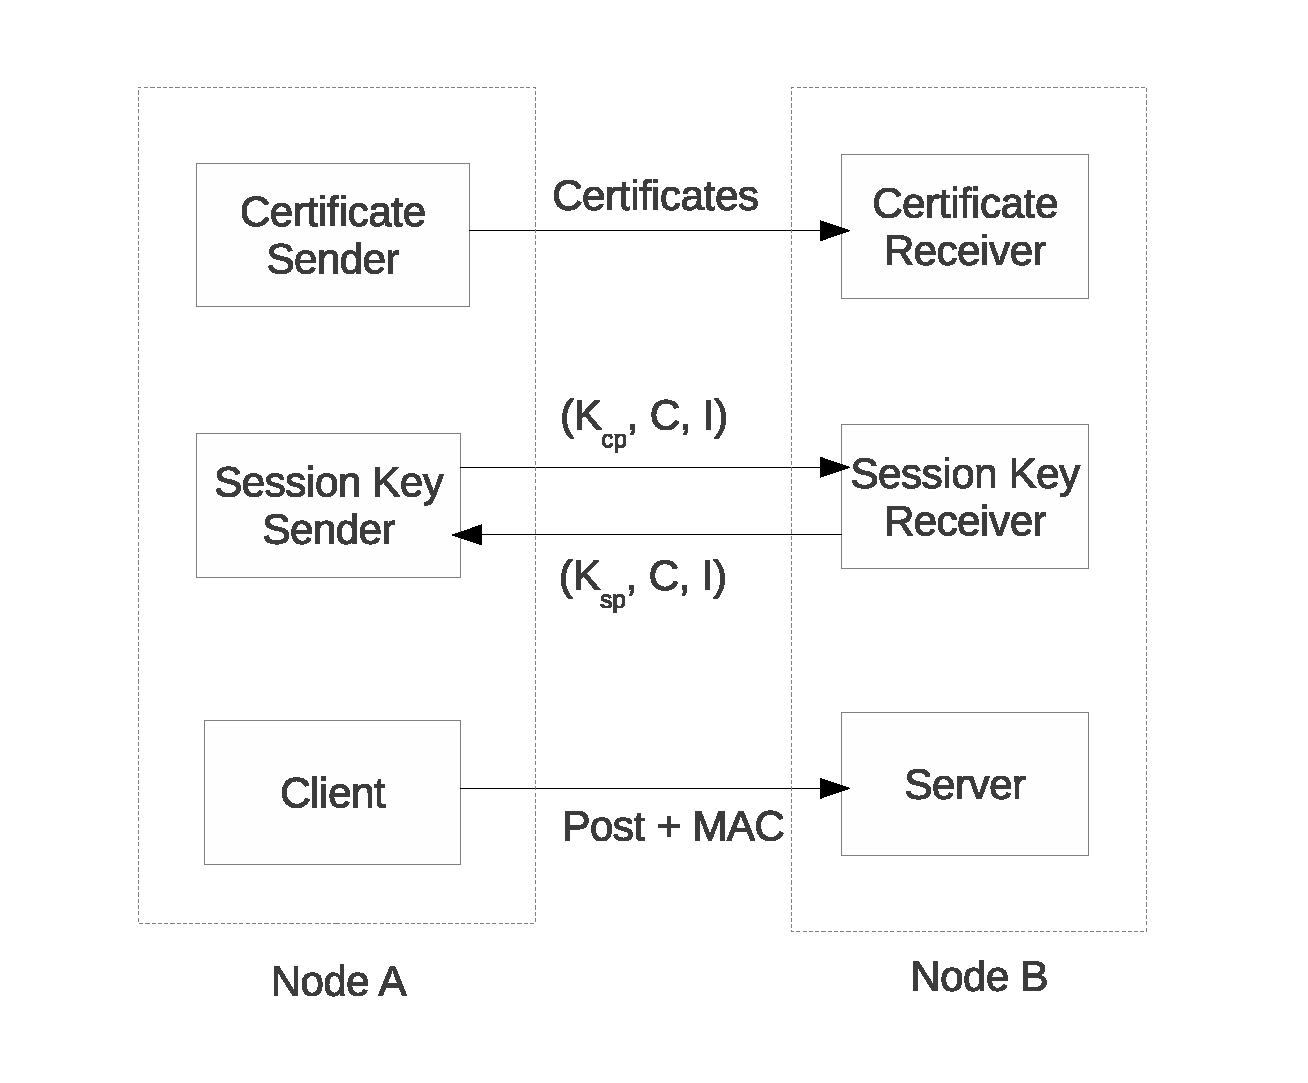
\includegraphics[scale=0.85]{SprocketRT-Protocol.eps}
\end{center}
\stopslide

\startslide{Maximum Message Transfer Rate}
\begin{center}
  \newcommand\T{\rule{0pt}{2.1ex}}
  \begin{tabular}{|l|r|r|} \hline
    \textit{Test} \T & \textit{messages/s} & \textit{\% Reduction} \\
    \hline \hline

    Baseline \T & 128 &   -- \\ \hline 
    Duties   \T & 119 &  7.0 \\ \hline
    MAC      \T &  87 & 32.0 \\ \hline
  \end{tabular}
\end{center}

The MAC was computed using hardware assisted AES on the nodes.

(Tmote Sky, 16KiB RAM, 48KiB ROM, 8MHz MSP430, TinyOS 2.1.2)
\stopslide

\startslide{Processing Time for Transient Operations}
\begin{center}
  \newcommand\T{\rule{0pt}{2.1ex}}
  \begin{tabular}{|l|r|} \hline
    \textit{Operation} \T & \textit{Time} \\ \hline \hline

    Certificate Verification     \T &  82s \\ \hline 
    Minimum Model Construction   \T & 370$\mu$s \\ \hline
    Session Key Negotiation      \T &  80s\\ \hline
  \end{tabular}
\end{center}

Minimum model time depends on complexity of policy, number of credentials, etc.

Test above used a set of five credentials, simulating a reasonable policy.
\stopslide

\startslide{General Observations}
\begin{citemize}
\item At boot long delays due to certificate processing.
\item At first post long delays due to session key negotiation (many posts lost initially).
\item Performance good after start-up.
\item Periodic posts from a node advance as a \textit{slow wave}.
\end{citemize}
\stopslide

%% SCALANESS!

\startslide{Staged Approach}

\begin{citemize}
\item Split computations into two stages!
\item Heavy crypto in first stage on powerful base stations.
\item Negotiated keys burned into second stage on nodes.
\item \cemph{Scalaness}: First stage language based on Scala.
\item \cemph{Mininess/nesT}: Second stage language based on nesC.
\end{citemize}

Scalaness is a modified Scala compiler that manipulates Mininess components

\begin{center}
\url{https://github.com/pchapin/scala}
\end{center}

(paper accepted at GPCE 2013)
\stopslide

\startslide{Scalaness Example}
\begin{lstlisting}[language=scalaness]
// A component for computing checksums.
@ModuleType(
"""{}
   < checksumType <: UInt32; size: UInt16 >
   { ; checksum(data: Array[UInt8]): checksumType }""")
class ChecksumC extends MininessComponent {
  "ChecksumC.nc"
}

...

@ModuleType("""{ checksumType <: UInt32 }<;>{ ; }""")
val resultModule =
  LibraryIC +>
    getChecksummer(desiredChecksumType, desiredSize) +>
       LibraryEC

resultModule.image()
\end{lstlisting}
\stopslide

\startslide{Types as Values}
\begin{lstlisting}[language=scalaness]
def getChecksumType(args: Array[String]) = {
  args(0).toInt match {
    case  8 => 
      println("Selecting 8 bit checksums")   
      new MetaType(UInt8)
        
    case 16 =>
      println("Selecting 16 bit checksums") 
      new MetaType(UInt16)

    case 32 =>
      println("Selecting 32 bit checksums")
      new MetaType(UInt32)
  }
}
\end{lstlisting}
\stopslide

\startslide{More Observations}
\begin{citemize}
\item Of course Scalaness is allows more optimized node programs!
\item Type safety is retained, even across stages (all generated programs will type check).
\item \cemph{Scalaness is general!}
\end{citemize}
\stopslide

\startslide{Conclusion}

Scalaness/nesT is a two-stage language for WSN programming and orchestration.

\begin{citemize}
\item Orchestrating program written in Scala variany, run on powerful hub
\item Second-stage code is efficient TinyOS program
\item Allows factoring of public and private key computations in secure SpartanRPC 
applications
\begin{citemize}
\item Expensive operations offloaded to orchestrating hub
\end{citemize} 
\item Other interesting applications for automated, ``intelligent'' network 
control.
\end{citemize}

\stopslide


\end{document}
